\documentclass[tikz,border=2pt]{standalone}

\usepackage{amsmath}
\usepackage{xcolor}
\usepackage{tikz}
\usetikzlibrary{arrows.meta,positioning,fit,backgrounds,calc,decorations.pathreplacing,patterns,shapes.geometric}
\usepackage{pgfplots}
\pgfplotsset{compat=1.18}
\usepgfplotslibrary{groupplots,fillbetween}

\definecolor{bestcolor}{HTML}{E8F5E9}
\definecolor{gaincolor}{HTML}{1B5E20}
\definecolor{cStandard}{HTML}{BF616A}
\definecolor{cAOI}{HTML}{5E81AC}
\definecolor{cDelta}{HTML}{A3BE8C}
\definecolor{cVisual}{HTML}{D08770}
\definecolor{cASR}{HTML}{B48EAD}
\definecolor{cNarr}{HTML}{88C0D0}
\definecolor{cAccent}{HTML}{EBCB8B}
\definecolor{cGray}{HTML}{4C566A}
\definecolor{cLightGray}{HTML}{D8DEE9}

\begin{document}
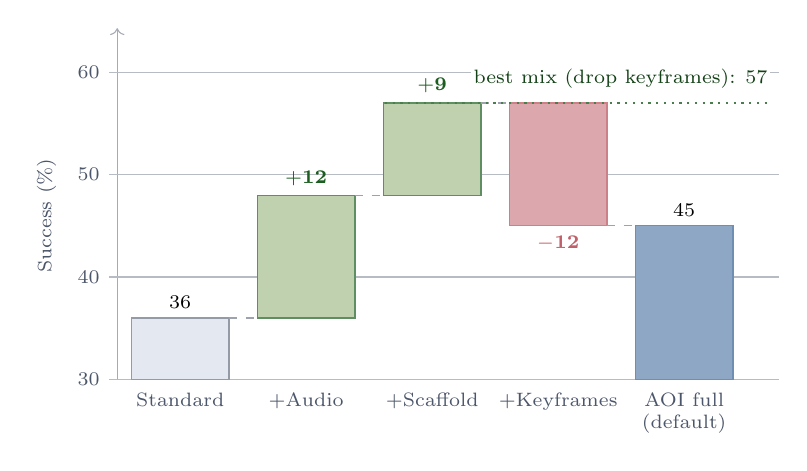
\begin{tikzpicture}[font=\small]
  \def\yb{30}\def\ys{0.13}\def\bw{0.62}
  \draw[cGray!50,->] (0.2,0) -- (0.2,{(62-\yb)*\ys+0.3});
  \foreach \v in {30,40,50,60} {
    \draw[cGray!40] (0.1,{(\v-\yb)*\ys}) -- (8.6,{(\v-\yb)*\ys});
    \node[font=\scriptsize,text=cGray,anchor=east] at (0.1,{(\v-\yb)*\ys}) {\v};
  }
  \node[font=\scriptsize,text=cGray,rotate=90,anchor=south] at (-0.45,{(46-\yb)*\ys}) {Success (\%)};
  \draw[fill=cLightGray!70,draw=cGray!60] (1-\bw,0) rectangle (1+\bw,{(36-\yb)*\ys});
  \node[font=\scriptsize,anchor=south] at (1,{(36-\yb)*\ys}) {36};
  \node[font=\scriptsize,text=cGray,align=center,anchor=north] at (1,-0.05) {Standard};
  \draw[fill=cDelta!70,draw=gaincolor!70] (2.6-\bw,{(36-\yb)*\ys}) rectangle (2.6+\bw,{(48-\yb)*\ys});
  \node[font=\scriptsize\bfseries,text=gaincolor,anchor=south] at (2.6,{(48-\yb)*\ys}) {$+$12};
  \node[font=\scriptsize,text=cGray,align=center,anchor=north] at (2.6,-0.05) {$+$Audio};
  \draw[fill=cDelta!70,draw=gaincolor!70] (4.2-\bw,{(48-\yb)*\ys}) rectangle (4.2+\bw,{(57-\yb)*\ys});
  \node[font=\scriptsize\bfseries,text=gaincolor,anchor=south] at (4.2,{(57-\yb)*\ys}) {$+$9};
  \node[font=\scriptsize,text=cGray,align=center,anchor=north] at (4.2,-0.05) {$+$Scaffold};
  \draw[fill=cStandard!55,draw=cStandard!80] (5.8-\bw,{(45-\yb)*\ys}) rectangle (5.8+\bw,{(57-\yb)*\ys});
  \node[font=\scriptsize\bfseries,text=cStandard,anchor=north] at (5.8,{(45-\yb)*\ys}) {$-$12};
  \node[font=\scriptsize,text=cGray,align=center,anchor=north] at (5.8,-0.05) {$+$Keyframes};
  \draw[fill=cAOI!70,draw=cAOI!90] (7.4-\bw,0) rectangle (7.4+\bw,{(45-\yb)*\ys});
  \node[font=\scriptsize,anchor=south] at (7.4,{(45-\yb)*\ys}) {45};
  \node[font=\scriptsize,text=cGray,align=center,anchor=north] at (7.4,-0.05) {AOI full\\(default)};
  \draw[cGray!55,dashed] (1+\bw,{(36-\yb)*\ys}) -- (2.6-\bw,{(36-\yb)*\ys});
  \draw[cGray!55,dashed] (2.6+\bw,{(48-\yb)*\ys}) -- (4.2-\bw,{(48-\yb)*\ys});
  \draw[cGray!55,dashed] (4.2+\bw,{(57-\yb)*\ys}) -- (5.8-\bw,{(57-\yb)*\ys});
  \draw[cGray!55,dashed] (5.8+\bw,{(45-\yb)*\ys}) -- (7.4-\bw,{(45-\yb)*\ys});
  \draw[gaincolor!80,thick,dotted] (3.6,{(57-\yb)*\ys}) -- (8.5,{(57-\yb)*\ys});
  \node[font=\scriptsize,text=gaincolor!70!black,anchor=east,fill=white,inner sep=1pt]
     at (8.5,{(59.4-\yb)*\ys}) {best mix (drop keyframes): 57};
\end{tikzpicture}
\end{document}
